\documentclass[aspectratio=169, xcolor=table]{beamer}
\usepackage[magyar]{babel}
\usepackage{t1enc}
\usepackage{lipsum}

\begin{document}

    \begin{frame}
        \title{Cím dia}
        \subtitle{Cím dia alcíme}
        
        \maketitle
    \end{frame}

    \begin{frame}{Cím}{Alcím}
        \begin{columns}[t]
            \begin{column}{.5\linewidth}
                \begin{itemize}
                    \item pont
                    \item pontpont
                \end{itemize}
                
                \begin{enumerate}
                    \item első
                    \item második
                    \item harmadik
                \end{enumerate}
            \end{column}
            
            \begin{column}{.5\linewidth}
                \begin{figure}
                    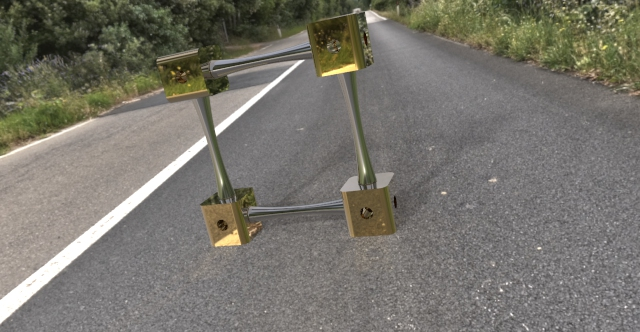
\includegraphics[keepaspectratio, width=5cm]{8. Lesson/creo.jpg}
                    \caption{Kép}
                \end{figure}
            \end{column}
        \end{columns}
    \end{frame}
    
    \begin{frame}{Blokkok}
        \begin{block}
            cím nélkül
        \end{block}
        
        \begin{block}{sima}
            kék
        \end{block}
        
        \begin{exampleblock}{példa}
            zöld
        \end{exampleblock}
        
        \begin{alertblock}{figyelmeztető}
            piros
        \end{alertblock}
    \end{frame}
    
    \begin{frame}{Theorem, proof}
        \begin{theorem}
            Pitagorasz tétele...
        \end{theorem}
        
        \begin{proof}[Pitagorasz tétel bizonyítása]
            Készítsünk két darab... \qedhere
        \end{proof}
    \end{frame}
    
    \begin{frame}{Semiverbatim}
        \begin{semiverbatim}
            Lista kódja:
            
                \\begin\{enumerate\}
                
                    \textcolor{red}{\\item egy}
                    
                    \\begin\{itemize\}
                    
                        \textcolor{blue}{\\item második szint}
                        
                    \\end\{itemize\}
                    
                    \\item kettő
                    
                \\end\{enumerate\}
        \end{semiverbatim}
    \end{frame}
    
\end{document}